\documentclass[11pt,a4paper,spanish]{book}
\usepackage{estilo_unir-1}
\usepackage{apacite}

\usepackage{hyperref}
\numberwithin{equation}{chapter}
\numberwithin{figure}{chapter}
\numberwithin{table}{chapter}


%---------------------------
% Título del trabajo y autor
%---------------------------
\title{Sistema de Asistencia Conversacional con LLM y Knowledge Graph para Warhammer: The Old World}
\tfetitulo{Sistema de Asistencia Conversacional con LLM y Knowledge Graph para Warhammer: The Old World}
% NOTA: se define el título dos veces a propósito.
% \title{...} alimenta los metadatos del PDF a través de hyperref.
% \tfetitulo{...} es la macro que realmente se usa en portada y cabecera,
% ya que \thetitle (paquete titling) deja de ser fiable en el cuerpo del
% documento al chocar con la redefinición de \title que hace hyperref.
\titulacion{Máster Universitario en Inteligencia Artificial}
\author{Eloy Rubiños Alonso}
\date{PENDIENTE: día de mes de 2026} % fecha de depósito/predepósito
\director{María de las Mercedes Barrachina Fernández}
\nombreciudad{Lugo}

%---------------------------
% Márgenes
%---------------------------
%\usepackage[margin=1.9cm]{geometry}


\begin{document}
\renewcommand{\listfigurename}{Índice de Ilustraciones}
\renewcommand{\listtablename}{Índice de Tablas}
\renewcommand{\contentsname}{Índice de Contenidos}
\renewcommand{\figurename}{Figura}
\renewcommand{\tablename}{Tabla}

\maketitle

\frontmatter
\tableofcontents
\listoffigures
\listoftables

%==================================================
% RESUMEN
%==================================================
\chapter{Resumen}

Warhammer: The Old World es un juego de miniaturas de mesa cuyo reglamento se compone de cientos de reglas especiales, miles de perfiles de unidad y un extenso conjunto de aclaraciones oficiales (FAQ) y erratas, todo ello entrelazado mediante referencias cruzadas. Responder con precisión a una consulta reglamentaria habitual exige combinar información dispersa en varias páginas. Esta es una tarea que los sistemas de generación aumentada por recuperación (RAG) convencionales, basados en similitud vectorial sobre fragmentos de texto independientes, resuelven mal cuando la pregunta requiere varios saltos de razonamiento. Este trabajo aborda esa limitación mediante el diseño y desarrollo de un sistema de asistencia conversacional basado en una arquitectura GraphRAG: una combinación de búsqueda semántica vectorial y recorrido de un grafo de conocimiento, pensada para resolver consultas reglamentarias con citación verificable de la fuente y para asistir en la construcción de listas de ejército legales.

La metodología combinó la extracción automatizada del contenido de la wiki comunitaria \emph{tow.whfb.app} mediante un crawler propio, el modelado de ese contenido en un grafo de conocimiento en Neo4j (conforme a un esquema diseñado para este dominio concreto) y la posterior construcción de un pipeline de recuperación híbrido, orquestado mediante LangChain/LangGraph, sobre un modelo de lenguaje Anthropic (Claude). El desarrollo siguió una metodología Kanban y las decisiones de arquitectura quedaron documentadas mediante Architecture Decision Records.

El sistema extrajo y estructuró la totalidad del contenido reglamentario disponible en la fuente, en un grafo de \texttt{TODO: nº final de nodos} nodos y \texttt{TODO: nº final de aristas} relaciones, e implementó sobre él un pipeline GraphRAG con citación de fuente verificable junto con un módulo de asistencia a la construcción de listas de ejército. La validación, realizada con \texttt{TODO: nº final de jugadores (mínimo 5)} jugadores reales de Warhammer: The Old World, obtuvo una precisión de citación del \texttt{TODO: \%}, una tasa de acierto en las respuestas del \texttt{TODO: \%} y una puntuación media de utilidad en escala Likert de \texttt{TODO: puntuación sobre 5}; \texttt{TODO: confirmar si se alcanzó o no el objetivo de >4/5 fijado en el Capítulo 3}. A partir de estos resultados puede concluirse que \texttt{TODO: conclusión principal del trabajo, una vez analizados los resultados de la validación}.

{\bf Palabras clave:} grafo de conocimiento, recuperación aumentada por generación, modelos de lenguaje, sistemas conversacionales, Warhammer: The Old World.


%==================================================
% MAINMATTER
%==================================================
\mainmatter

%==================================================
% CAPÍTULO 1 - INTRODUCCIÓN
%==================================================
\chapter{Introducción}

El resto del capítulo presenta el contexto que motiva el desarrollo de este trabajo, plantea de forma general la solución propuesta y describe la organización del resto del documento. Se parte de una necesidad concreta identificada en la comunidad de jugadores de Warhammer: The Old World, se justifica por qué las técnicas actuales de generación aumentada por recuperación resultan insuficientes para cubrirla, y se anticipa el enfoque híbrido grafo-vectorial que se desarrolla en los capítulos siguientes.

\section{Motivación}

Warhammer: The Old World es un juego de miniaturas de mesa publicado por Games Workshop que recupera y amplía el sistema de reglas clásico de Warhammer Fantasy Battle. Su reglamento incluye diecinueve facciones jugables, cada una con sus propias unidades, reglas especiales, hechizos y restricciones de composición de listas, todo ello sobre un núcleo de reglas comunes que regula el movimiento, el combate y la magia. Esta complejidad no es accidental: forma parte del diseño del juego y constituye buena parte de su atractivo estratégico. Pero también es la causa de un problema práctico bien conocido por sus jugadores. Responder con precisión a una pregunta de reglas habitual (por ejemplo, qué ocurre cuando una unidad con la regla Regeneración recibe daño de un ataque con la regla Llameante) exige localizar y combinar correctamente varias reglas especiales, comprobar si existe alguna aclaración oficial (FAQ) o errata que modifique su interacción, y aplicar esa combinación al caso concreto planteado. Esta tarea de resolución de reglas interrelacionadas, en la que la respuesta correcta no reside en un único pasaje del reglamento sino en la combinación de varios, se conoce en la literatura de procesamiento del lenguaje natural como razonamiento multi-hop o multi-salto.

Los modelos de lenguaje de gran escala (LLM) y, en particular, la técnica de generación aumentada por recuperación o RAG \citeA{lewis2020rag}, han permitido construir asistentes conversacionales capaces de responder preguntas sobre corpus documentales específicos sin reentrenar el modelo. Sin embargo, los sistemas RAG convencionales recuperan fragmentos de texto mediante similitud vectorial entre la pregunta y los documentos indexados. Esto funciona razonablemente bien cuando la respuesta está contenida en un único fragmento, pero presenta limitaciones notables cuando hay que combinar información dispersa en varios documentos relacionados entre sí \cite{peng2024graphragsurvey}. Es justamente esta limitación la que afecta a los sistemas existentes de consulta de reglas para juegos de mesa: en su práctica totalidad emplean RAG vectorial plano sobre el texto del reglamento, sin modelar las relaciones entre reglas, unidades y excepciones.

Frente a esto ha emergido, en los últimos años, la técnica conocida como GraphRAG, que combina la recuperación semántica vectorial con el recorrido de un grafo de conocimiento que representa las entidades del dominio y sus relaciones \cite{edge2024graphrag}. Trabajos recientes en dominios igualmente caracterizados por una densa interrelación normativa --como el razonamiento jurídico multi-salto o la consulta de normativa de seguridad en construcción-- han demostrado mejoras sustanciales de precisión y exhaustividad al introducir un grafo de conocimiento frente a enfoques puramente vectoriales \cite{bifrostrag2025}. Esta evidencia, junto con la ausencia de trabajos previos que apliquen GraphRAG al dominio de los wargames de mesa, es la motivación central de este trabajo: comprobar si esa misma ventaja se reproduce en un dominio de reglas de juego con una estructura de interdependencias comparable a la de los dominios normativos ya estudiados.

\section{Planteamiento del trabajo}

A partir de la necesidad descrita, este trabajo plantea el diseño, desarrollo y validación de un sistema de asistencia conversacional para Warhammer: The Old World construido sobre una arquitectura GraphRAG. El sistema se alimenta de un grafo de conocimiento construido de forma automatizada a partir del contenido de la wiki comunitaria \emph{tow.whfb.app}, que funciona como fuente única de reglas, unidades, ejércitos, hechizos, objetos mágicos y aclaraciones oficiales del juego.

Cubre dos capacidades complementarias. Por un lado, la resolución de consultas reglamentarias en lenguaje natural, devolviendo una respuesta que cita la página o páginas de origen de la información empleada para que el jugador pueda verificarla contra la fuente oficial. Por otro, la asistencia en la construcción de listas de ejército: sugerir unidades y advertir de restricciones de composición, presupuesto de puntos o reglas de alianza entre facciones. Ambas capacidades comparten la misma infraestructura de grafo de conocimiento y el mismo motor de recuperación híbrida, de modo que el razonamiento sobre relaciones estructurales del dominio se reutiliza entre los dos casos de uso. El Capítulo 3 desarrolla los objetivos concretos derivados de este planteamiento, formulados de manera específica, medible, alcanzable, relevante y con un horizonte temporal definido.

\section{Estructura del trabajo}

El resto del documento se organiza en seis capítulos adicionales. El Capítulo 2 sitúa el estado del arte en generación aumentada por recuperación, GraphRAG y aplicaciones de modelos de lenguaje a dominios reglamentarios complejos. El Capítulo 3 formula los objetivos del trabajo y describe la metodología seguida. El Capítulo 4 recoge el proceso de identificación de requisitos. En el Capítulo 5 se describe la herramienta software desarrollada: arquitectura, tecnologías, proceso de extracción y modelado de datos, estado de implementación. Los Capítulos 6 y 7 cierran el documento con la validación del sistema con usuarios reales y las conclusiones del trabajo, respectivamente, junto con las líneas de trabajo futuro que abre.


%==================================================
% CAPÍTULO 2 - CONTEXTO Y ESTADO DEL ARTE
%==================================================
\chapter{Contexto y estado del arte}

Este capítulo sitúa el trabajo dentro de su contexto de aplicación y revisa la literatura científica relevante. Primero se describe el problema desde la perspectiva del dominio: los wargames de mesa con reglamentos extensos. Después se repasa el estado del arte en tres líneas: la generación aumentada por recuperación y sus límites conocidos, su extensión mediante grafos de conocimiento, y las aplicaciones existentes de modelos de lenguaje a dominios con alta densidad de reglas interrelacionadas. El capítulo cierra enlazando lo revisado con la contribución concreta de los capítulos siguientes.

\section{Contexto del problema}

Los juegos de miniaturas de mesa como Warhammer: The Old World pertenecen a una categoría de productos lúdicos con reglamentos extensos, repartidos a menudo en varios documentos (reglas núcleo, manuales de ejército, suplementos, FAQ y erratas) que se actualizan periódicamente. Esta fragmentación, sumada a que las reglas están interconectadas entre sí (una regla especial puede modificar el comportamiento de otra, una errata puede alterar el texto original de una unidad, una restricción de lista puede depender de varias reglas de ejército a la vez), genera fricción real para el jugador que necesita resolver una duda durante una partida o preparar una lista legal antes de jugar.

Esto no es exclusivo de Warhammer: The Old World. Comunidades de jugadores de otros juegos con reglamentos complejos han desarrollado herramientas de consulta basadas en IA, casi siempre mediante RAG aplicado directamente sobre el texto del reglamento \cite{boardgameguru2023}. Funcionan bien para consultas que dependen de un único pasaje, pero no incorporan mecanismos de razonamiento estructurado sobre las relaciones entre reglas, que es justo el problema que aborda este trabajo. La wiki comunitaria \emph{tow.whfb.app}, empleada como fuente de datos, resulta especialmente favorable aquí: a diferencia del texto en prosa de un manual impreso, estructura el contenido en páginas individuales por entidad de juego (unidad, regla, hechizo, objeto mágico) enlazadas mediante hiperenlaces, lo que facilita convertirlo directamente en un grafo de conocimiento sin tener que extraer relaciones de texto no estructurado.

\section{Estado del arte}

\subsection{Generación aumentada por recuperación: fundamentos y limitaciones}

La generación aumentada por recuperación, o RAG, fue propuesta por \citeA{lewis2020rag} como método para combinar el conocimiento parametrizado de un modelo de lenguaje preentrenado con una memoria no parametrizada: un índice vectorial denso sobre una colección de documentos externos. Un modelo de lenguaje convencional responde solo a partir de lo aprendido durante el entrenamiento; un sistema RAG, en cambio, recupera en tiempo de consulta los fragmentos más similares semánticamente a la pregunta del usuario y los incorpora como contexto adicional en la generación de la respuesta. Esto reduce de forma notable la generación de contenido fabricado o "alucinado" por el modelo, al anclar la respuesta a fuentes verificables, y permite aplicar modelos de lenguaje a dominios privados o específicos sin reentrenamiento.

La recuperación vectorial sobre la que se apoya el RAG convencional representa tanto la consulta como los fragmentos del corpus como vectores de alta dimensionalidad mediante un modelo de embeddings, de modo que la similitud semántica entre textos se aproxima mediante una medida de distancia vectorial (habitualmente la similitud coseno). La familia Sentence-BERT \cite{reimers2019sbert} consolidó este enfoque al introducir una red siamesa sobre BERT, optimizada para producir embeddings de oraciones comparables mediante operaciones vectoriales simples; antes de eso, los enfoques requerían procesar cada par de textos conjuntamente, algo computacionalmente inviable a la escala de un corpus de recuperación.

Pese a estas ventajas, el RAG vectorial tiene una limitación estructural. Cuando la respuesta a una consulta no está contenida en un único fragmento del corpus, sino que requiere combinar información de varios fragmentos relacionados entre sí (lo que se conoce como razonamiento multi-hop o multi-salto), el sistema no tiene ningún mecanismo para identificar que dos fragmentos recuperados por separado deben combinarse. Tampoco puede descubrir un tercer fragmento relevante que no sea semánticamente similar a la consulta original pero sí esté relacionado con los ya recuperados \cite{peng2024graphragsurvey}. A esto se suma algo más grave: los estudios sobre fidelidad y atribución en sistemas RAG han encontrado que una proporción relevante de las respuestas generadas contiene afirmaciones sin respaldo verificable en los documentos recuperados. Esto afecta directamente al objetivo de citación precisa de fuentes que es uno de los pilares de este trabajo \cite{attributionsurvey2026}.

\subsection{GraphRAG: recuperación aumentada con grafos de conocimiento}

Como respuesta a las limitaciones del RAG vectorial en razonamiento multi-salto, ha emergido en los últimos años la técnica conocida como GraphRAG, que incorpora un grafo de conocimiento explícito como estructura intermedia entre el corpus documental y el proceso de generación. \citeA{edge2024graphrag} proponen, en uno de los trabajos fundacionales de esta línea, construir un grafo de entidades y relaciones a partir del corpus mediante un modelo de lenguaje, agruparlo en comunidades jerárquicas con algoritmos de detección de comunidades, y generar resúmenes precomputados de cada comunidad. Esto permite responder preguntas globales de síntesis sobre todo el corpus con una reducción sustancial del coste computacional respecto a procesar el texto fuente completo en cada consulta.

\citeA{peng2024graphragsurvey} formalizan el flujo de trabajo de los sistemas GraphRAG en tres etapas: indexación basada en grafo (construir y enriquecer el grafo a partir del corpus), recuperación guiada por grafo (seleccionar subgrafos relevantes combinando señales vectoriales y estructurales) y generación potenciada por grafo (incorporar el subgrafo recuperado como contexto estructurado para el modelo de lenguaje). Esta taxonomía es directamente aplicable al sistema de este trabajo: la indexación corresponde a la construcción del grafo de conocimiento del Capítulo 5, y la recuperación y generación al pipeline GraphRAG descrito en el mismo capítulo.

Hay, sin embargo, una diferencia relevante respecto al enfoque de \citeA{edge2024graphrag}: el origen del grafo de conocimiento. Su propuesta extrae el grafo de un corpus de texto no estructurado mediante un modelo de lenguaje, lo que introduce una fuente adicional de error e incertidumbre en la construcción. Este trabajo, en cambio, aprovecha que la fuente de datos --la wiki comunitaria \emph{tow.whfb.app}-- ya presenta una estructura semi-estructurada, con entidades de juego diferenciadas (unidades, reglas, hechizos) e hiperenlaces entre ellas. Esa característica permite construir un grafo de mayor precisión mediante extracción estructurada directa, sin depender de que un modelo de lenguaje infiera correctamente las relaciones del dominio a partir de texto libre.

\subsection{GraphRAG en dominios reglamentarios complejos}

La aplicación de GraphRAG a dominios con alta densidad de reglas interrelacionadas ha empezado a explorarse en ámbitos normativos distintos al de los wargames de mesa, con resultados que respaldan la hipótesis de partida de este trabajo. En el ámbito jurídico, los sistemas de razonamiento legal multi-salto que combinan un grafo de conocimiento normativo con recuperación vectorial muestran mejoras sustanciales de precisión frente a la recuperación vectorial pura, en preguntas que requieren combinar varias disposiciones legales relacionadas mediante remisiones y excepciones \cite{legalgraphrag2026}.

Un caso particularmente cercano al planteamiento de este trabajo es BifrostRAG \cite{bifrostrag2025}: un sistema que construye dos grafos de conocimiento complementarios (uno de relaciones lingüísticas y otro de estructura documental) a partir de normativa de seguridad en construcción, con el objetivo de responder preguntas multi-salto sobre dicha normativa. Evaluado sobre noventa y tres preguntas multi-salto, obtuvo una precisión del 92,8\%, una exhaustividad del 85,5\% y una puntuación F1 del 87,3\%, superando con significación estadística tanto a un sistema de RAG vectorial puro como a uno de GraphRAG de grafo único. Este resultado importa por dos razones. Confirma, en un dominio normativo de complejidad comparable a un reglamento de wargame, que un grafo de conocimiento estructurado mejora de forma medible la resolución de consultas multi-salto frente a la recuperación vectorial. Y, además, ofrece un precedente metodológico (preguntas multi-salto anotadas, métricas de precisión, exhaustividad y F1) que informa el diseño del protocolo de validación de este trabajo, descrito en el Capítulo 6.

Las herramientas de consulta de reglas existentes para juegos de mesa, en cambio, como las descritas por \citeA{boardgameguru2023}, se limitan casi por completo a una arquitectura de RAG vectorial plano sobre el texto del reglamento, sin modelar las relaciones entre reglas, unidades y excepciones que sí han demostrado aportar valor en los dominios normativos anteriores. Esa ausencia de precedentes que apliquen GraphRAG al dominio de los wargames de mesa es el vacío de investigación que este trabajo se propone explorar.

\section{Conclusiones}

La revisión de la literatura confirma que el RAG vectorial convencional, aunque eficaz en general para anclar las respuestas de un modelo de lenguaje a fuentes documentales verificables, tiene una limitación conocida en tareas de razonamiento multi-salto sobre información distribuida en varios documentos relacionados. GraphRAG, al incorporar un grafo de conocimiento explícito como estructura intermedia, ha demostrado en dominios normativos de complejidad comparable a un reglamento de wargame --el jurídico, el de la normativa técnica de seguridad-- mejoras medibles de precisión y exhaustividad frente a la recuperación puramente vectorial. No se ha encontrado, sin embargo, ningún trabajo previo que aplique esta técnica al dominio específico de los reglamentos de juegos de miniaturas de mesa, donde las herramientas existentes siguen apoyándose en RAG vectorial plano.

Esa combinación, evidencia favorable en dominios análogos y ausencia de antecedentes en el dominio de aplicación, es la base que justifica la contribución de este trabajo: diseñar, desarrollar y validar un sistema GraphRAG aplicado específicamente al reglamento de Warhammer: The Old World, aprovechando además una característica distintiva de la fuente de datos empleada (su estructura semi-estructurada con hiperenlaces entre entidades de juego) que permite construir el grafo de conocimiento mediante extracción estructurada directa, sin depender de inferir relaciones a partir de texto libre. El Capítulo 3 formula los objetivos concretos derivados de esta motivación.


%==================================================
% CAPÍTULO 3 - OBJETIVOS Y METODOLOGÍA DE TRABAJO
%==================================================
\chapter{Objetivos concretos y metodología de trabajo}

Lo que sigue conecta el estudio del dominio y el estado del arte del capítulo anterior con la contribución concreta que se desarrolla más adelante. Primero se formula el objetivo general, seguido de los objetivos específicos que lo concretan, todos definidos según el criterio SMART --específico, medible, alcanzable, relevante y temporalmente delimitado-- propuesto por \citeA{doran1981}. Después se describe la metodología de trabajo: las fases del proyecto, las herramientas empleadas en cada una y el procedimiento previsto para analizar los resultados.

\section{Objetivo general}

Desarrollar un sistema de asistencia conversacional basado en una arquitectura GraphRAG sobre un grafo de conocimiento construido a partir de la wiki comunitaria \emph{tow.whfb.app}, capaz de resolver consultas reglamentarias del juego Warhammer: The Old World con citación verificable de fuentes y de asistir en la construcción de listas de ejército legales.

\section{Objetivos específicos}

A partir del objetivo general se derivan los siguientes objetivos específicos, formulados con verbo en infinitivo y orientados a un resultado observable y verificable:

\begin{itemize}
	\item \textbf{Extraer y estructurar} el corpus completo de reglas, unidades, ejércitos y entidades de juego de \emph{tow.whfb.app} en un grafo de conocimiento en Neo4j, alcanzando una cobertura verificada superior al 95\% de las páginas indexadas en los inventarios oficiales del sitio (sitemaps y tabla de contenidos).
	\item \textbf{Diseñar y documentar} mediante Architecture Decision Records las decisiones estructurales del sistema --selección de base de datos, estrategia de crawling, contrato de datos y convenciones de almacenamiento--, garantizando la trazabilidad y justificación técnica de cada decisión.
	\item \textbf{Implementar} un pipeline GraphRAG que combine búsqueda vectorial semántica mediante embeddings multilingües con recorrido de grafo, para resolver consultas reglamentarias multi-salto a través de una interfaz conversacional con citación de fuente (URL) en cada respuesta.
	\item \textbf{Desarrollar} un módulo de asistencia a la construcción de listas de ejército que aplique las restricciones de composición, presupuesto de puntos y reglas de alianza codificadas en el grafo de conocimiento.
	\item \textbf{Validar} la utilidad y precisión del sistema mediante una prueba con un mínimo de cinco jugadores reales de Warhammer: The Old World, midiendo la precisión de citación, la tasa de acierto en las respuestas y la percepción de utilidad en escala Likert, con el objetivo de alcanzar una puntuación media superior a 4 sobre 5.
\end{itemize}

\section{Metodología del trabajo}

El desarrollo siguió una metodología de tipo Kanban, que permite ver el flujo de tareas en curso, pendientes y completadas, y ajustar prioridades sobre la marcha a medida que el conocimiento del dominio y de las restricciones técnicas de la fuente de datos se iba refinando durante el propio trabajo. Esta elección encaja bien con un proyecto individual de naturaleza exploratoria como este: varias decisiones iniciales tuvieron que revisarse a la luz de hallazgos técnicos no anticipados al empezar (como se documenta en el Capítulo 5), algo que una metodología de fases cerradas tipo cascada habría obligado a replanificar de forma mucho más rígida.

El trabajo se organiza en cuatro fases, alineadas con los objetivos específicos de la sección anterior.

Primero viene la extracción y estructuración de los datos: diseño e implementación de un crawler que recorre la totalidad de las páginas de \emph{tow.whfb.app} mediante búsqueda en anchura con semillas múltiples, desarrollo de parsers especializados por tipo de contenido (unidades, reglas, hechizos, objetos mágicos, FAQ, erratas, entre otros) y modelado del resultado en un grafo de conocimiento en Neo4j conforme a un esquema diseñado para este dominio. Las decisiones técnicas de esta fase --motor de base de datos, arquitectura del crawler, estrategia de obtención de datos, convenciones de almacenamiento en el grafo-- quedaron documentadas mediante Architecture Decision Records, siguiendo una práctica de ingeniería de software que favorece la trazabilidad frente a las alternativas consideradas.

Después se enriquece el grafo de conocimiento generando representaciones vectoriales (embeddings) de los nodos relevantes e incorporando traducciones al español; esta es la infraestructura de recuperación semántica sobre la que se apoya el pipeline conversacional.

A continuación se implementa el pipeline GraphRAG propiamente dicho --recuperación vectorial y recorrido de grafo mediante LangChain/LangGraph sobre un modelo de lenguaje configurable-- junto con la interfaz conversacional que lo expone al usuario final, incluido el módulo de asistencia a la construcción de listas de ejército.

Por último se valida el sistema con un mínimo de cinco jugadores reales de Warhammer: The Old World. El protocolo, detallado en el Capítulo 6, combina métricas cuantitativas (precisión de la citación de fuentes y tasa de acierto en las respuestas frente a un conjunto de preguntas de referencia) con valoraciones cualitativas de utilidad y usabilidad mediante un cuestionario Likert de cinco puntos, siguiendo un esquema de evaluación inspirado en trabajos previos de aplicación de GraphRAG a dominios normativos complejos \cite{bifrostrag2025}.


%==================================================
% CAPÍTULO 4 - IDENTIFICACIÓN DE REQUISITOS
%==================================================
\chapter{Identificación de requisitos}

El presente capítulo recoge el trabajo previo de identificación de requisitos que ha guiado las decisiones de diseño del sistema descrito en el Capítulo 5. La identificación de requisitos de un sistema de asistencia conversacional para un juego de mesa con un reglamento tan extenso como el de Warhammer: The Old World tiene una particularidad respecto a un proyecto de software convencional: gran parte de los requisitos funcionales no vienen de una especificación de negocio, sino de las propias características del dominio de juego y de las necesidades habituales de sus jugadores. Se han identificado a partir de la experiencia del autor como jugador de Warhammer: The Old World, del análisis de la estructura y contenido de la fuente de datos empleada, y de la revisión de herramientas comunitarias existentes para juegos de mesa de complejidad reglamentaria comparable.

Los dos casos de uso que motivan el trabajo, descritos en el Capítulo 1, marcan directamente buena parte de los requisitos funcionales. El sistema tiene que responder consultas en lenguaje natural sobre reglas, unidades, hechizos, objetos mágicos y restricciones de ejército, citando la página de origen de la wiki comunitaria en la que se basa cada afirmación, para que el jugador pueda verificar la respuesta contra la fuente oficial sin tener que confiar a ciegas en el sistema. También tiene que resolver consultas que combinan información de varias entidades relacionadas entre sí (una regla especial cuyo efecto se ve modificado por una errata, o una unidad cuya elegibilidad para un objeto mágico depende a la vez de su tipo de tropa y de su facción), que es el requisito que diferencia este sistema de un RAG vectorial convencional y justifica la arquitectura GraphRAG. Y, por último, debe asistir en la construcción de listas de ejército aplicando automáticamente las restricciones de composición porcentual, presupuesto de puntos por categoría y reglas de alianza entre facciones que el reglamento impone sobre cualquier lista legal.

Otro conjunto de requisitos viene de cómo está organizada la fuente de datos. La wiki \emph{tow.whfb.app} estructura su contenido en páginas diferenciadas por tipo de entidad de juego (ejércitos, unidades, reglas especiales, reglas núcleo, hechizos, objetos mágicos, tipos de tropa, terreno, FAQ y erratas), enlazadas mediante hiperenlaces que en muchos casos son relaciones semánticamente significativas para el dominio --por ejemplo, un enlace desde el texto de una unidad hacia la página de una regla especial que esa unidad posee--. De ahí se deriva un requisito concreto: el sistema de extracción tiene que distinguir el tipo de contenido de cada página y capturar tanto sus atributos propios como sus relaciones con otras entidades, para que dichas relaciones puedan convertirse en aristas explícitas en el grafo de conocimiento en lugar de perderse en una representación puramente textual.

La naturaleza académica e individual del proyecto impone, además, requisitos de carácter no funcional. El sistema tiene que poder desarrollarse y ejecutarse con herramientas gratuitas o de uso libre, sin costes de infraestructura cloud que no sean asumibles para un trabajo de fin de máster individual; esto condicionó, por ejemplo, la elección de Neo4j Community Edition (autoalojable en un único nodo) frente a alternativas con licencias comerciales o servicios gestionados de pago. También debe respetar las condiciones de uso de la fuente de datos --verificadas consultando el archivo \texttt{robots.txt} del sitio-- y limitar la frecuencia de las peticiones durante la extracción para no sobrecargar la infraestructura de la wiki comunitaria. Y como la wiki fuente está en inglés mientras que la comunidad hispanohablante de jugadores es un público objetivo relevante, el sistema necesita responder consultas en español sin mantener manualmente una traducción completa de todo el corpus, lo que llevó a adoptar un modelo de embeddings multilingüe capaz de relacionar consultas en español con contenido fuente en inglés.

Finalmente, la propia normativa de evaluación de la Universidad Internacional de La Rioja para los Trabajos de Fin de Máster de tipo desarrollo de software exige justificar documentalmente las decisiones de arquitectura y validar la herramienta con usuarios reales del dominio. Esto se ha traducido en la práctica de documentación sistemática mediante Architecture Decision Records mantenida durante todo el desarrollo, y en el diseño del protocolo de validación con un mínimo de cinco jugadores reales descrito en el Capítulo 6.


%==================================================
% CAPÍTULO 5 - DESCRIPCIÓN DE LA HERRAMIENTA SOFTWARE DESARROLLADA
%==================================================
\chapter{Descripción de la herramienta software desarrollada}

En las páginas que siguen se describe la herramienta software desarrollada durante este trabajo: su arquitectura general, las tecnologías empleadas en cada componente, y el proceso de extracción y modelado de los datos que alimentan el grafo de conocimiento. Las decisiones de arquitectura más relevantes se presentan junto con las alternativas consideradas y el razonamiento que llevó a su selección, siguiendo la práctica de documentación mediante Architecture Decision Records adoptada durante todo el desarrollo.

\section{Arquitectura general del sistema}

El sistema se organiza en cuatro bloques que se ejecutan de forma secuencial: un pipeline de datos que extrae y estructura el contenido de la wiki comunitaria \emph{tow.whfb.app}, un grafo de conocimiento en Neo4j que almacena de forma persistente ese contenido junto con sus relaciones e índices vectoriales, un backend que implementa el pipeline de recuperación híbrida GraphRAG y expone una API conversacional, y un frontend web con la interfaz de usuario tanto para la consulta conversacional como para la visualización del grafo. La Figura \ref{fig:arquitectura-general} resume esta organización.

\begin{figure}[h]
\centering
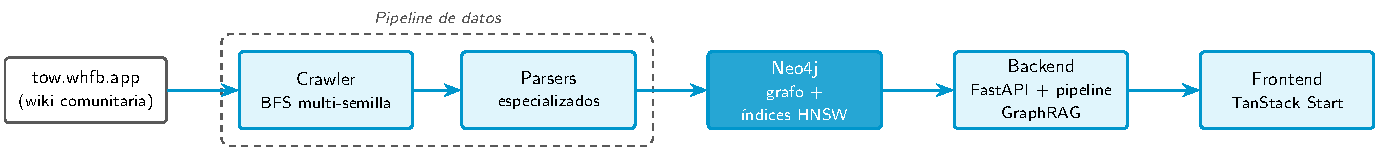
\includegraphics[width=0.95\textwidth]{arquitectura_general}
\caption{Arquitectura general del sistema, desde la fuente de datos hasta la interfaz de usuario}
\label{fig:arquitectura-general}
{\footnotesize\centering Fuente: elaboración propia.\par}
\end{figure}

El pipeline de datos es responsable de la extracción, estructuración y enriquecimiento del grafo, y se detalla en la Sección \ref{sec:pipeline-datos}. El backend y el frontend, encargados respectivamente del pipeline GraphRAG y de la interfaz conversacional, se describen en las Secciones \ref{sec:backend} y \ref{sec:frontend}.

\section{Pila tecnológica}

La selección de tecnologías se ha realizado de forma diferenciada para cada componente del sistema, atendiendo a los requisitos identificados en el Capítulo 4 y, en los casos de mayor relevancia arquitectónica, documentando la decisión mediante un Architecture Decision Record. La Tabla \ref{tab:stack-pipeline} resume las tecnologías empleadas en el pipeline de extracción y modelado de datos.

\begin{table}[h]
\centering
\begin{tabular}{|p{3.3cm}|p{3.3cm}|p{5.7cm}|}
	\hline
	\textbf{Componente} & \textbf{Tecnología} & \textbf{Notas} \\
	\hline
	Lenguaje & Python 3.11+ & Tipado estático mediante type hints \\
	\hline
	Gestor de paquetes & \texttt{uv} & Preferido frente a pip/poetry \\
	\hline
	Cliente HTTP & \texttt{requests} & HTML estático; no requiere navegador headless \\
	\hline
	Parsing HTML & \texttt{beautifulsoup4} & Para tablas de estadísticas en el DOM renderizado \\
	\hline
	Extracción JSON & \texttt{json} (estándar) & Parsea el bloque \texttt{\_\_NEXT\_DATA\_\_} embebido \\
	\hline
	Linter & \texttt{ruff} & Longitud de línea 100 \\
	\hline
	Tests & \texttt{pytest} & Unitarios e integración \\
	\hline
\end{tabular}
\caption{Pila tecnológica del pipeline de datos}
\label{tab:stack-pipeline}
{\footnotesize\centering Fuente: elaboración propia.\par}
\end{table}

La Tabla \ref{tab:stack-grafo} resume la pila tecnológica correspondiente a la base de datos de grafo y a la generación de embeddings.

\begin{table}[h]
\centering
\begin{tabular}{|p{2.8cm}|p{3.8cm}|p{5.7cm}|}
	\hline
	\textbf{Componente} & \textbf{Tecnología} & \textbf{Notas} \\
	\hline
	Base de datos de grafo & Neo4j Community Edition 5.24 & Desplegado mediante Docker \\
	\hline
	Despliegue & Docker Compose & Plugin APOC requerido para tipos de relación dinámicos \\
	\hline
	Driver Python & \texttt{neo4j} (oficial) & Carga por lotes mediante \texttt{MERGE} e \texttt{UNWIND} \\
	\hline
	Búsqueda vectorial & \texttt{db.index.vector.queryNodes} (nativo de Neo4j) & Invocado directamente vía el driver oficial \texttt{neo4j}, no mediante el paquete \texttt{neo4j-graphrag}; recuperación híbrida (vectorial + texto completo, fusión por Reciprocal Rank Fusion) y recorrido de grafo implementados a medida -- justificación en el ADR-0009 \\
	\hline
	Índice vectorial & HNSW nativo de Neo4j 5.x & Un índice por etiqueta, 768 dimensiones, similitud coseno \\
	\hline
	Modelo de embeddings & {\fontsize{8}{9.5}\selectfont\texttt{paraphrase-}\newline\texttt{multilingual-}\newline\texttt{mpnet-base-v2}} & \texttt{sentence-transformers}; arquitectura derivada de Sentence-BERT \cite{reimers2019sbert} \\
	\hline
\end{tabular}
\caption{Pila tecnológica de la base de datos de grafo y los embeddings}
\label{tab:stack-grafo}
{\footnotesize\centering Fuente: elaboración propia.\par}
\end{table}

La Tabla \ref{tab:stack-backend-frontend} resume la pila tecnológica empleada en el backend y el frontend.

\begin{table}[h]
\centering
\begin{tabular}{|p{3.3cm}|p{3.3cm}|p{5.7cm}|}
	\hline
	\textbf{Componente} & \textbf{Tecnología} & \textbf{Notas} \\
	\hline
	Framework backend & FastAPI + uvicorn & API REST \\
	\hline
	Proveedores LLM & Anthropic (Claude) & Resuelto mediante \texttt{api/dependencies.py::get\_llm()}, configurable sobre OpenAI / Anthropic / Ollama mediante la variable de entorno \texttt{LLM\_PROVIDER}; ver justificación en el texto \\
	\hline
	Streaming & Vercel AI SDK (formato SSE) & Helper dedicado en el backend \\
	\hline
	Orquestación & LangChain / LangGraph & Construcción del pipeline de recuperación y generación \\
	\hline
	Framework frontend & TanStack Start & Renderizado híbrido SSR/SPA con rutas basadas en ficheros \\
	\hline
	Estilos & Tailwind CSS v4 & \\
	\hline
	Componentes UI & HeroUI & \\
	\hline
	Arquitectura frontend & Feature-Sliced Design & Separación explícita entre la funcionalidad de chat y la de visualización del grafo \\
	\hline
\end{tabular}
\caption{Pila tecnológica del backend y el frontend}
\label{tab:stack-backend-frontend}
{\footnotesize\centering Fuente: elaboración propia.\par}
\end{table}

\section{Fuente de datos y extracción}
\label{sec:pipeline-datos}

\subsection{La fuente de datos: tow.whfb.app}

La fuente de datos empleada es \emph{tow.whfb.app}, una wiki comunitaria de uso educativo que indexa el reglamento completo de Warhammer: The Old World, incluyendo las diecinueve facciones jugables --Beastmen Brayherds, Chaos Dwarfs, Daemons of Chaos, Dark Elves, Dwarfen Mountain Holds, Empire of Man, Grand Cathay, High Elf Realms, Kingdom of Bretonnia, Lizardmen, Ogre Kingdoms, Orc \& Goblin Tribes, Realms of Men, Regiments of Renown, Skaven, Tomb Kings of Khemri, Vampire Counts, Warriors of Chaos y Wood Elf Realms-- junto con las reglas núcleo, reglas especiales, hechizos, objetos mágicos, tipos de tropa y los documentos oficiales de aclaraciones (FAQ) y erratas. Antes de empezar el desarrollo del crawler se verificó la conformidad de la extracción con el archivo \texttt{robots.txt} del sitio, que permite el acceso a la totalidad de las páginas de contenido y solo restringe rutas internas no relevantes para este trabajo (\texttt{/api/*}, \texttt{/apps/*} y \texttt{/regenerate}). El crawler se identifica mediante una cabecera de \emph{user-agent} propia (\texttt{WarhawmerTOW-GraphRAG-Thesis/1.0}) para que el tráfico generado sea trazable.

Una decisión técnica condicionó de forma significativa el diseño del crawler y de los parsers, y quedó documentada como una adenda al ADR-0002: el sitio no se sirve como HTML renderizado por servidor en el sentido tradicional, sino que está construido sobre Next.js con Contentful como sistema de gestión de contenidos headless, con las páginas pre-renderizadas mediante regeneración estática incremental. Cada página HTML incluye, embebido en una etiqueta \texttt{script} con identificador \texttt{\_\_NEXT\_DATA\_\_}, la respuesta completa de Contentful para esa entrada, con todas las entradas enlazadas y los documentos de texto enriquecido ya resueltos en tiempo de construcción. No se anticipó esto en la planificación inicial del proyecto, pero simplificó bastante la arquitectura de extracción: no hace falta un navegador headless de tipo Playwright o Puppeteer, porque todo el contenido estructurado es accesible mediante una petición HTTP estándar seguida de una extracción de expresión regular y un \texttt{json.loads()} sobre dicho bloque.

\subsection{Arquitectura del crawler}

El crawler implementa una estrategia de búsqueda en anchura con semillas múltiples, documentada en el ADR-0002. Usa tres inventarios de URL complementarios entre sí: la tabla de contenidos de la wiki, que enumera todas las secciones de reglas y las diecinueve páginas de ejército junto con las páginas de FAQ y erratas; el índice alfabético \texttt{/sitemap/rules}, que recoge de forma exhaustiva más de 1.500 páginas individuales de reglas; y el índice alfabético \texttt{/sitemap/armies}, que recoge la totalidad de las páginas de unidad bajo el patrón \texttt{/unit/\{slug\}}. La necesidad de combinar estas tres semillas se comprobó en la práctica: una estrategia basada solo en la tabla de contenidos no habría descubierto ninguna de las 574 páginas de unidad, porque no están enlazadas directamente desde dicha tabla, y una basada solo en los sitemaps habría omitido las páginas de FAQ y erratas, que no aparecen en ninguno de los dos índices alfabéticos.

Como medida de cortesía hacia la infraestructura del sitio fuente, el crawler aplica un retardo mínimo configurable entre peticiones consecutivas (un segundo por defecto), y normaliza y deduplica las URL descubiertas para que cada página se solicite exactamente una vez. Se ejecuta una única vez y persiste los resultados en disco; no hay peticiones a la wiki en tiempo de consulta del sistema conversacional. También se evaluó, conforme al ADR-0003, complementar o sustituir los datos extraídos con los ficheros JSON de proyectos comunitarios de código abierto similares, como Old World Builder. Se descartó tras comprobar que todos los datos necesarios (estadísticas, costes en puntos, texto íntegro de reglas especiales, reglas de composición de ejército, objetos mágicos y erratas, estas últimas ya integradas en el cuerpo de las páginas de la wiki) están disponibles directamente en el HTML de la wiki. Esos ficheros JSON, además, no aportan los hiperenlaces entre páginas que son la base de las aristas del grafo de conocimiento.

\subsection{Resultado de la extracción}

La ejecución completa del crawler sobre la totalidad del sitio ha producido 3.260 páginas HTML almacenadas en bruto, distribuidas por categoría de contenido conforme a la Tabla \ref{tab:scraping-metricas}.

\begin{table}[h]
\centering
\begin{tabular}{|l|r|}
	\hline
	\textbf{Categoría de contenido} & \textbf{Páginas extraídas} \\
	\hline
	Reglas núcleo & 1.535 \\
	\hline
	Reglas especiales & 643 \\
	\hline
	Unidades & 574 \\
	\hline
	Armas & 264 \\
	\hline
	Objetos mágicos & 70 \\
	\hline
	Tipos de tropa & 40 \\
	\hline
	Secciones de FAQ & 39 \\
	\hline
	Hechizos (páginas dedicadas) & 38 \\
	\hline
	Terreno & 37 \\
	\hline
	Ejércitos & 19 \\
	\hline
	Errata & 1 \\
	\hline
	\textbf{Total} & \textbf{3.260} \\
	\hline
\end{tabular}
\caption{Páginas extraídas de tow.whfb.app por categoría de contenido}
\label{tab:scraping-metricas}
{\footnotesize\centering Fuente: elaboración propia, a partir de la ejecución del crawler sobre la totalidad del sitio. \texttt{TODO: re-verificar cifra final antes del depósito.}\par}
\end{table}

Cada página extraída se enruta, en función del tipo de contenido Contentful identificado en su bloque \texttt{\_\_NEXT\_DATA\_\_} y del patrón de su URL, hacia el parser especializado correspondiente: \texttt{ArmyParser} para las páginas de tipo \texttt{association} (\texttt{/army/\{slug\}}), \texttt{UnitParser} para las páginas de tipo \texttt{armyListEntry} (\texttt{/unit/\{slug\}}), y un conjunto de parsers especializados --\texttt{RuleParser}, \texttt{CoreRuleParser}, \texttt{SpellParser}, \texttt{MagicItemParser}, \texttt{WeaponParser} y \texttt{LoreParser}-- para el resto de páginas de tipo \texttt{rule}, diferenciadas entre sí por el patrón de su URL. Esta fase de extracción y parsing se encuentra completa y verificada, con los dieciocho ficheros JSON resultantes (uno por tipo de nodo, más un fichero adicional de aristas) almacenados en el directorio \texttt{data/parsed/} del repositorio del proyecto.

\subsection{Parsing híbrido: datos estructurados y tablas renderizadas}

Durante el desarrollo se identificó que determinados atributos críticos para resolver consultas de juego --en particular, las estadísticas de armas (alcance, fuerza, valor de penetración de armadura) y los metadatos de hechizos (valor de lanzamiento, alcance, tipo)-- no estaban en los campos estructurados de Contentful, sino que solo se generan en la tabla de estadísticas renderizada en el HTML de la página. Esto, documentado en el ADR-0006, llevó a un enfoque de parsing híbrido: los datos estructurados de Contentful se usan como fuente principal, combinados con una extracción mediante BeautifulSoup sobre las tablas de estadísticas del mismo fichero HTML ya descargado, sin necesidad de una nueva petición HTTP ni de un navegador headless. También se detectó y corrigió un problema de enrutado por el que las páginas dedicadas de hechizos (\texttt{/spell/\{slug\}}) se procesaban con el parser genérico de reglas núcleo, generando colisiones de identificador entre nodos de hechizo y de regla núcleo; tras corregirlo, los 139 hechizos del corpus tienen los atributos \texttt{spell\_type} y \texttt{casting\_value}, y esas colisiones desaparecieron.

\section{Grafo de conocimiento}

\subsection{Principios de diseño}

El esquema del grafo de conocimiento, en su versión 3.0 definitiva tras una revisión completa frente a los dos casos de uso del sistema, se apoya en varios principios de diseño aplicados de forma consistente. El inglés es el idioma canónico para todos los campos estructurales y textos de origen; las traducciones al español se añaden como propiedades escalares independientes con el sufijo \texttt{\_es} (por ejemplo, \texttt{name\_es}, \texttt{text\_es}), sin tocar la estructura del grafo. La búsqueda multilingüe se resuelve con el modelo de embeddings \texttt{paraphrase-multilingual-mpnet-base-v2}, que proyecta consultas en español a la misma región del espacio vectorial que los nodos en inglés, así que no hace falta mantener vectores separados por idioma. Neo4j solo admite propiedades de nodo de tipo escalar o listas homogéneas de escalares, de modo que cualquier normalización de estructuras anidadas presentes en los datos de origen (como las coordenadas de cita bibliográfica o las dimensiones de base de una miniatura) se resuelve en la fase de parsing, antes de la carga al grafo, dejando el cargador como una etapa de \texttt{MERGE} puro sin lógica de transformación. Los subperfiles estadísticos de una unidad (por ejemplo, los perfiles diferenciados de jinete y montura) se modelan como nodos \texttt{:Profile} de primer orden conectados mediante aristas \texttt{HAS\_PROFILE}, en lugar de como una propiedad de tipo lista de objetos: esto permite hacer consultas Cypher de comparación directa sobre los valores estadísticos.

\subsection{Esquema de nodos y relaciones}

El grafo construido contiene diecisiete tipos de nodo, recogidos en la Tabla \ref{tab:grafo-nodos}, con un total de 7.789 nodos.

\begin{table}[h]
\centering
{\fontsize{9}{11}\selectfont
\begin{tabular}{|l|r|p{6.5cm}|}
	\hline
	\textbf{Etiqueta} & \textbf{Cantidad} & \textbf{Descripción} \\
	\hline
	Army & 19 & Facciones jugables \\
	\hline
	Unit & 574 & Unidades, personajes, monturas \\
	\hline
	Profile & 945 & Subperfiles estadísticos (jinete/montura/campeón) \\
	\hline
	SpecialRule & 643 & Reglas universales, de ejército y únicas \\
	\hline
	CoreRule & 1.377 & Páginas de mecánicas del reglamento \\
	\hline
	Document & 37 & Páginas de orientación sin valor de traversal \\
	\hline
	TroopType & 40 & Definiciones de tipo de tropa, con datos de bonificación por rango \\
	\hline
	Lore & 38 & Lores de magia \\
	\hline
	Spell & 139 & Hechizos individuales \\
	\hline
	Weapon & 264 & Armas, armadura y equipo \\
	\hline
	MagicItem & 698 & Objetos mágicos universales y de ejército \\
	\hline
	FAQ & 244 & Entradas oficiales de preguntas frecuentes \\
	\hline
	Errata & 210 & Correcciones oficiales de errata \\
	\hline
	Upgrade & 2.424 & Opciones de mejora adquiribles por unidad \\
	\hline
	CompositionList & 17 & Estructura de listas de composición de ejército \\
	\hline
	CompositionSlot & 83 & Restricciones de hueco de composición \\
	\hline
	Terrain & 37 & Categorías y elementos de terreno \\
	\hline
	\textbf{Total} & \textbf{7.789} & \\
	\hline
\end{tabular}
}
\caption{Tipos de nodo del grafo de conocimiento}
\label{tab:grafo-nodos}
{\footnotesize\centering Fuente: elaboración propia, a partir de métricas del grafo en ejecución. \texttt{TODO: re-verificar cifras finales antes del depósito.}\par}
\end{table}

Por encima de los nodos, veintisiete tipos de relación (sumando aproximadamente 92.011 aristas) materializan tanto enlaces explícitos extraídos de los hiperenlaces de la wiki como relaciones derivadas calculadas tras la carga del grafo. La Tabla \ref{tab:grafo-aristas} recoge las relaciones más numerosas y su significado en el dominio.

\begin{table}[h]
\centering
{\fontsize{9}{11}\selectfont
\begin{tabular}{|l|r|p{6.5cm}|}
	\hline
	\textbf{Tipo de relación} & \textbf{Cantidad} & \textbf{Semántica} \\
	\hline
	CAN\_TAKE\_ITEM & 69.942 & Unidad $\rightarrow$ objeto mágico que puede adquirir (derivada) \\
	\hline
	REFERENCES & 6.031 & Referencia cruzada entre reglas a partir de hiperenlaces \\
	\hline
	HAS\_RULE & 4.395 & Unidad $\rightarrow$ regla especial siempre activa \\
	\hline
	HAS\_UPGRADE & 2.433 & Unidad $\rightarrow$ mejora adquirible \\
	\hline
	HAS\_PROFILE & 967 & Unidad $\rightarrow$ nodo de perfil estadístico \\
	\hline
	HAS\_WEAPON & 1.607 & Unidad $\rightarrow$ arma de equipo estándar \\
	\hline
	BELONGS\_TO & 595 & Unidad $\rightarrow$ ejército \\
	\hline
	CLARIFIES & 510 & FAQ $\rightarrow$ nodo aclarado \\
	\hline
	AMENDS & 407 & Errata $\rightarrow$ nodo corregido \\
	\hline
	ALLIED\_WITH & 44 & Ejército $\rightarrow$ ejército aliado, con tipo de alianza \\
	\hline
	\textbf{Total (27 tipos)} & \textbf{$\sim$92.011} & \\
	\hline
\end{tabular}
}
\caption{Principales tipos de relación del grafo de conocimiento}
\label{tab:grafo-aristas}
{\footnotesize\centering Fuente: elaboración propia, a partir de métricas del grafo en ejecución. \texttt{TODO: re-verificar cifras finales antes del depósito.}\par}
\end{table}

Las 69.942 aristas \texttt{CAN\_TAKE\_ITEM} no se generan directamente durante el parsing: se materializan en una etapa posterior a la carga del grafo mediante tres pasadas idempotentes de \texttt{MERGE} basadas en el tipo de mejora, el nivel de hechicero y la afiliación de ejército de cada unidad. Esta decisión, documentada en el ADR-0005, parte de que esa relación de elegibilidad estructural puede derivarse de forma determinista a partir de propiedades ya presentes en el grafo, sin duplicar esa lógica durante el parsing. Eso sí, la relación captura solo la elegibilidad estructural; restricciones expresadas en prosa dentro del reglamento, como no poder repetir un objeto mágico de la misma categoría en una misma lista, no se codifican en el grafo y quedan delegadas a la capa de aplicación.

\subsection{Indexación vectorial}

Sobre doce de los diecisiete tipos de nodo --Army, Unit, SpecialRule, CoreRule, Document, TroopType, Spell, MagicItem, Lore, Weapon, FAQ y Errata-- se creó un índice vectorial HNSW independiente por etiqueta, de 768 dimensiones y similitud coseno, con embeddings generados a partir del modelo \texttt{paraphrase-multilingual-mpnet-base-v2}. Tener un índice por etiqueta en lugar de uno único global permite acotar la búsqueda por similitud a un subconjunto semánticamente relevante de nodos: por ejemplo, restringirla a nodos de tipo \texttt{SpecialRule} cuando la consulta es sobre una regla concreta, en vez de buscar sobre todos los nodos del grafo. El texto de cada embedding no es una serialización directa del JSON de origen, sino que se enriquece con el contexto de los nodos vecinos tras la carga del grafo; así, el texto embebido para una unidad incluye también sus reglas especiales y su equipo asociado.

\subsection{Métricas de calidad del grafo}

Se han calculado un conjunto de métricas de calidad sobre el grafo cargado, recogidas en la Tabla \ref{tab:grafo-calidad}, con el objetivo de verificar la cobertura e integridad de las relaciones derivadas de fuentes oficiales de aclaración y corrección del reglamento.

\begin{table}[h]
\centering
\begin{tabular}{|p{7cm}|r|}
	\hline
	\textbf{Métrica} & \textbf{Valor} \\
	\hline
	Entradas de FAQ con arista CLARIFIES & 203 / 244 (83,2\%) \\
	\hline
	Entradas de errata con arista AMENDS & 185 / 210 (88,1\%) \\
	\hline
	Armas con \texttt{range} no nulo & 226 / 264 \\
	\hline
	Hechizos con \texttt{spell\_type} y \texttt{casting\_value} & 139 / 139 (100\%) \\
	\hline
	Aristas huérfanas (nodo origen ausente) & 3 (aceptadas, impacto menor) \\
	\hline
	Aristas huérfanas (nodo destino ausente) & 0 \\
	\hline
\end{tabular}
\caption{Métricas de calidad del grafo de conocimiento}
\label{tab:grafo-calidad}
{\footnotesize\centering Fuente: elaboración propia, a partir de la validación posterior a la carga del grafo. \texttt{TODO: re-verificar cifras finales antes del depósito.}\par}
\end{table}

Las brechas de cobertura de estas métricas, junto con otras lagunas de parsing conocidas y dejadas para más adelante --como la falta de presupuesto de objetos mágicos específico por perfil en las mejoras de campeón, o la ausencia de estadísticas de disparo para máquinas de guerra que se modelan como unidad en lugar de como arma-- están documentadas en el repositorio del proyecto como deuda técnica conocida, no como defectos sin identificar. \texttt{TODO: indicar si estas lagunas se priorizaron finalmente a la luz del impacto observado durante la validación con usuarios (Capítulo 6).}

\section{Backend: pipeline GraphRAG}
\label{sec:backend}

El backend implementa el pipeline de recuperación híbrida GraphRAG y lo expone mediante una API conversacional. Su estructura de directorios sigue dos restricciones de diseño explícitas. La primera: el proveedor de modelo de lenguaje se resuelve siempre a través de una función de resolución centralizada (\texttt{api/dependencies.py::get\_llm()}), configurable mediante la variable de entorno \texttt{LLM\_PROVIDER}, así que ninguna ruta de la API ni del pipeline de recuperación importa directamente un proveedor concreto; un módulo anterior (\texttt{llm/client.py}) que perseguía el mismo objetivo mediante una clase de abstracción quedó deprecado en favor de este mecanismo (ADR-0007). Esto permitió comparar proveedores --OpenAI, Anthropic u Ollama para inferencia local-- sin tocar el código de negocio durante la fase de evaluación, hasta seleccionar finalmente \textbf{Anthropic} (modelo \texttt{claude-sonnet-5} por defecto, configurable mediante \texttt{LLM\_MODEL}). La elección no fue por inercia: el mecanismo de citación verificable de fuentes --uno de los dos objetivos centrales de este trabajo (Sección 3.2)-- se apoya en bloques de contenido \texttt{search\_result} nativos de la API de Anthropic (\texttt{rag/tools.py::use\_native\_citations}), que permiten citas indexadas y verificables directamente por el modelo; ningún otro proveedor soportado ofrece un mecanismo equivalente. La segunda restricción de diseño: la lógica de negocio del pipeline de recuperación vive íntegramente en el módulo \texttt{rag/pipeline.py}, dejando los manejadores de ruta de la API como una capa fina de orquestación. A diferencia de lo previsto inicialmente (ADR-0001), el pipeline no se apoya en la clase \texttt{VectorCypherRetriever} del paquete \texttt{neo4j-graphrag}, sino en una implementación propia (\texttt{rag/retriever.py::GraphRAGRetriever}): búsqueda vectorial ANN mediante \texttt{db.index.vector.queryNodes} sobre un índice HNSW por etiqueta, con una modalidad híbrida opcional que fusiona los resultados vectoriales con búsqueda de texto completo (BM25) mediante Reciprocal Rank Fusion, combinada con un recorrido de grafo acotado (\texttt{rag/graph\_traversal.py::GraphTraversal}) para la expansión de contexto de un salto. La divergencia respecto al paquete oficial no fue una omisión sino una decisión evaluada explícitamente --incluyendo la revisión directa del código fuente de \texttt{neo4j-graphrag} para confirmar que sus clases de recuperación híbrida no ofrecen Reciprocal Rank Fusion (solo los rankers \texttt{NAIVE} y \texttt{LINEAR}) ni admiten múltiples índices vectoriales por etiqueta-- y queda documentada íntegramente en el ADR-0009. La respuesta se transmite al frontend mediante streaming por eventos del lado del servidor (SSE), compatible con el Vercel AI SDK.

\section{Frontend: interfaz conversacional y visualización del grafo}
\label{sec:frontend}

El frontend, responsable de la interfaz conversacional y de la visualización del grafo de conocimiento consultado en cada respuesta, se diseñó sobre TanStack Start: un framework que combina renderizado del lado del servidor con una aplicación de página única, organizado conforme al patrón arquitectónico Feature-Sliced Design. Esta elección responde a que la aplicación tiene dos funcionalidades claramente diferenciadas --la conversación con el sistema y la visualización del grafo-- que no comparten estado interno; las fronteras explícitas entre slices que impone Feature-Sliced Design, junto con las restricciones de importación verificadas en tiempo de análisis estático mediante Biome, permitieron detectar violaciones de ese acoplamiento de forma temprana durante el desarrollo. La interfaz de chat se apoya en el hook \texttt{useChat} del Vercel AI SDK para consumir la respuesta en streaming generada por el backend.

\section{Resumen de componentes desarrollados}

La Tabla \ref{tab:estado-implementacion} resume los componentes que conforman el sistema desarrollado, con indicación de los artefactos generados por cada uno.

\begin{table}[h]
\centering
\begin{tabular}{|l|p{8.5cm}|}
	\hline
	\textbf{Componente} & \textbf{Artefactos generados} \\
	\hline
	Extracción (scraping) & 3.260 páginas HTML en \texttt{data/raw/} \\
	\hline
	Parsing & 18 ficheros JSON en \texttt{data/parsed/} (uno por tipo de nodo, más aristas) \\
	\hline
	Construcción del grafo & Grafo de conocimiento en Neo4j (véase Tabla \ref{tab:grafo-nodos} para el desglose final de nodos y relaciones) \\
	\hline
	Embeddings e indexación vectorial & Índices vectoriales HNSW por etiqueta sobre doce tipos de nodo \\
	\hline
	Traducciones (i18n) & Propiedades \texttt{*\_es} pobladas para los campos de texto orientados al usuario \\
	\hline
	Backend (pipeline GraphRAG) & API REST en FastAPI con pipeline de recuperación híbrida \\
	\hline
	Frontend & Interfaz conversacional y de visualización del grafo en TanStack Start \\
	\hline
\end{tabular}
\caption{Componentes desarrollados y artefactos generados}
\label{tab:estado-implementacion}
{\footnotesize\centering Fuente: elaboración propia.\par}
\end{table}


%==================================================
% CAPÍTULO 6 - EVALUACIÓN
%==================================================
\chapter{Evaluación}
% Evaluación de usabilidad y aplicabilidad de la herramienta para resolver
% el problema propuesto. Habitualmente con usuarios expertos
% (objetivo de validación: ≥5 jugadores reales, escala Likert, métricas
% cuantitativas y cualitativas, precisión de citaciones, tasa de acierto en
% las respuestas, etc.).
%
% DECISIÓN DE ALCANCE (2026-06-22): se descarta la comparativa cuantitativa
% GraphRAG vs. RAG estándar como parte de la validación — estaba planteada
% como extra/opcional, no es viable en el tiempo disponible y es difícil de
% cuantificar con rigor. La validación con los ≥5 jugadores se centra en:
% (1) precisión de citación de fuentes, (2) tasa de acierto en las
% respuestas frente a un conjunto de preguntas de referencia, y (3)
% percepción de utilidad/usabilidad en escala Likert (objetivo >4/5). No
% hay condición de "RAG estándar" con la que comparar.
%
% NOTA SOBRE LA RÚBRICA: el criterio "Desarrollo específico de la
% contribución" (20%, el de mayor peso individual) distingue Notable de
% Sobresaliente principalmente por la presencia de una discusión de
% resultados clara, y no solo su descripción objetiva. Por ello se separa
% aquí la presentación de resultados de su interpretación, replicando el
% mismo patrón que las instrucciones UNIR exigen para los trabajos Tipo 1
% (piloto experimental), aunque no sea obligatorio para Tipo 2.
%
% PENDIENTE: este capítulo requiere los resultados reales de la validación
% con jugadores (Fase 4 de la metodología, Capítulo 3) y no se redacta en
% esta entrega parcial.

\section{Resultados}
% Presentación OBJETIVA de los resultados de la validación: tablas resumen
% de las puntuaciones Likert, precisión de citación de fuentes, tasa de
% acierto en las respuestas frente al conjunto de preguntas de referencia, y
% observaciones cualitativas recogidas. Sin valorar ni justificar los
% resultados todavía — esto se reserva a la sección siguiente.

\section{Discusión}
% Interpretación de los resultados anteriores: ¿qué significan?, ¿en qué
% medida el sistema resuelve satisfactoriamente las consultas multi-hop
% planteadas?, ¿qué datos anómalos aparecen y por qué?,
% limitaciones de la validación (tamaño de muestra, sesgos, etc.).


%==================================================
% CAPÍTULO 7 - CONCLUSIONES Y TRABAJO FUTURO
%==================================================
\chapter{Conclusiones y trabajo futuro}
% Resumen del problema tratado, cómo se ha abordado y por qué la solución
% sería válida.

\section{Conclusiones}
% Normativa UNIR + rúbrica (criterio "Relación entre objetivos,
% planteamiento, desarrollo y conclusiones", 10%): CADA objetivo específico
% planteado en el Capítulo 3 debe enlazarse aquí con una conclusión
% explícita. Se recomienda un mapeo uno a uno, por ejemplo:
%
% Objetivo específico 1 (Identificar...) -> Conclusión: se confirma que...
% Objetivo específico 2 (Desarrollar...)  -> Conclusión: se ha logrado...
% Objetivo específico 3 (Evaluar...)      -> Conclusión: los resultados
%                                             muestran que...
% [...]
%
% No basta con un resumen genérico: la rúbrica distingue explícitamente
% entre conclusiones que "responden a todos los objetivos" (Notable/
% Sobresaliente) y conclusiones que no lo hacen (Suspenso/Aprobado).
% Incluir también limitaciones del trabajo y, si aplica, una reflexión
% sobre la originalidad de las conclusiones (terminología propia, no solo
% reformulación de lo ya dicho en el desarrollo).

\section{Líneas de trabajo futuro}
% Perspectivas de futuro que abre el trabajo desarrollado para el campo de
% estudio. Justificar de qué modo y en qué campos puede emplearse la
% aportación realizada.


%==================================================
% REFERENCIAS BIBLIOGRÁFICAS
%==================================================
\addcontentsline{toc}{chapter}{Referencias bibliográficas}
\bibliographystyle{apacite}
\bibliography{bibliografia}


%==================================================
% ANEXOS
%==================================================
\appendix
\chapter{Código fuente y datos analizados}
% Incluir la URL del repositorio donde se aloja el código fuente desarrollado
% durante el TFE. El estudiante debe ser el único autor del código y único
% propietario del repositorio (sin commits de otros usuarios).
% Si el TFE está asociado a una actividad o proyecto de empresa, justificar
% aquí cualquier restricción de confidencialidad sobre código o datos.

\chapter{Declaración de uso de herramientas de inteligencia artificial}

En cumplimiento de la normativa de la Universidad Internacional de La Rioja sobre el uso de herramientas de inteligencia artificial (IA) generativa en la elaboración de Trabajos Fin de Estudios, se declara a continuación el uso realizado de estas herramientas durante el desarrollo del presente trabajo.

Durante la elaboración de este Trabajo Fin de Estudios se ha empleado el asistente de IA generativa Claude, desarrollado por Anthropic, en sus variantes Claude Opus 4.7 y Claude Opus 4.8 \cite{anthropic2026opus47, anthropic2026opus48} para tareas de planificación y análisis, y Claude Sonnet 4.5 y Claude Sonnet 4.6 \cite{anthropic2026sonnet45, anthropic2026sonnet46} para tareas de ejecución, como herramienta de apoyo en las siguientes tareas:

\begin{itemize}
	\item Asistencia en la revisión de estilo de determinados pasajes del documento, sobre contenido, estructura y decisiones técnicas aportadas íntegramente por el autor.
	\item Búsqueda y síntesis preliminar de bibliografía académica relacionada con generación aumentada por recuperación y GraphRAG, posteriormente verificada, seleccionada y referenciada por el autor.
	\item Generación de la figura de arquitectura del sistema (Figura \ref{fig:arquitectura-general}) a partir de las especificaciones de diseño aportadas por el autor.
	\item Apoyo puntual en la revisión de código LaTeX de la plantilla y en la depuración de errores de compilación.
    \item Apoyo en la generación de fragmentos de código del sistema a partir de especificaciones del autor, y en la depuración de código ya redactado por este, revisado en todos los casos antes de su incorporación al repositorio.
\end{itemize}

La totalidad de las decisiones de arquitectura, el diseño del esquema del grafo de conocimiento, la implementación del código fuente del proyecto y la verificación final de todo el contenido de esta memoria son responsabilidad exclusiva del autor, quien ha revisado, validado y, en su caso, corregido cada uno de los contenidos generados con apoyo de IA antes de su incorporación al documento. El uso de estas herramientas no ha sustituido en ningún caso el criterio técnico ni la autoría intelectual del trabajo, que corresponden íntegramente al autor.


%==================================================
% ÍNDICE DE ACRÓNIMOS (apartado opcional, UNIR 2.10)
%==================================================
\backmatter
\chapter*{Índice de acrónimos}
\addcontentsline{toc}{chapter}{Índice de acrónimos}

\noindent\textbf{ADR} -- Architecture Decision Record\\
\textbf{ANN} -- Approximate Nearest Neighbor (búsqueda aproximada de vecinos más próximos)\\
\textbf{APA} -- American Psychological Association\\
\textbf{API} -- Application Programming Interface\\
\textbf{CSS} -- Cascading Style Sheets\\
\textbf{FAQ} -- Frequently Asked Questions (preguntas frecuentes)\\
\textbf{GraphRAG} -- Graph-enhanced Retrieval-Augmented Generation\\
\textbf{HNSW} -- Hierarchical Navigable Small World (índice de búsqueda vectorial)\\
\textbf{HTML} -- HyperText Markup Language\\
\textbf{HTTP} -- HyperText Transfer Protocol\\
\textbf{IA} -- Inteligencia Artificial\\
\textbf{JSON} -- JavaScript Object Notation\\
\textbf{LLM} -- Large Language Model\\
\textbf{RAG} -- Retrieval-Augmented Generation\\
\textbf{SPA} -- Single Page Application\\
\textbf{SSE} -- Server-Sent Events\\
\textbf{SSR} -- Server-Side Rendering\\
\textbf{TFE} -- Trabajo Fin de Estudios\\
\textbf{TFM} -- Trabajo Fin de Máster\\
\textbf{UI} -- User Interface\\
\textbf{UNIR} -- Universidad Internacional de La Rioja\\
\textbf{URL} -- Uniform Resource Locator

\end{document}
